\documentclass[a4paper,oneside,brazil,11pt,a4paper,openright,titlepage,usenames,dvipsnames]{book}
% Classe alternativa, apropriada para impressão frente-verso. Inclui páginas em branco de forma que capítulos sempre tenham início na página à direita:
% \documentclass[11pt,a4paper,openright,titlepage]{book}

\usepackage[utf8]{inputenc}
\usepackage[T1]{fontenc}
\usepackage[brazilian]{babel}
\usepackage{lmodern}
\usepackage{array}
\usepackage{verbatim}
\usepackage{calc}
\usepackage{textcomp}
\usepackage{gensymb}
\usepackage{amsfonts}
\usepackage{amsmath}
\usepackage[thmmarks,amsmath]{ntheorem}%\usepackage{amsthm}
\usepackage{amssymb}
\usepackage{graphicx}
\usepackage{float}
\usepackage[]{subfigure}
\usepackage{epsfig}
\usepackage{boxedminipage}
\usepackage{geometry}
\usepackage{theorem}
\usepackage{fancybox}
\usepackage{fancyhdr}
\usepackage{ifthen}
\usepackage{url}
\usepackage{afterpage}
\usepackage{color}
\usepackage{colortbl}
\usepackage{rotating}
\usepackage{makeidx}
\usepackage{indentfirst}
\usepackage{import}
\usepackage{enumitem}

\usepackage{ft2unb}

\makeindex

\makeatother

\begin{document}
\setcounter{secnumdepth}{3}
\setcounter{tocdepth}{2}
\pagestyle{empty}

\grau{Engenheiro de Controle e Automação}

\tipodemonografia{TRABALHO DE GRADUAÇÃO}

% Título
\titulolinhai{RISC-V SiMPLE}
\titulolinhaii{}
\titulolinhaiii{}
\titulolinhaiv{}


% Autores
\autori{Arthur de Matos Beggs}
\autorii{}
\autoriii{}


% Membros da banca
\membrodabancai{Prof.\ Marcus Vinicius Lamar, CIC/UnB}
\membrodabancaifuncao{Orientador}

\membrodabancaii{Prof.\ Ricardo Pezzuol Jacobi, CIC/UnB}
\membrodabancaiifuncao{Co-Orientador}

\membrodabancaiii{}
\membrodabancaiiifuncao{}

\membrodabancaiv{}
\membrodabancaivfuncao{}

\membrodabancav{}
\membrodabancavfuncao{}


% Data de defesa
\mes{Julho}
\ano{2019}


% Comandos para criar a capa e a página de assinaturas
\capaprincipal{}
\capaassinaturas{}


% Ficha Catalográfica
\noindent \textbf{FICHA CATALOGRÁFICA}

\noindent %
\fbox{\begin{minipage}[t]{1\columnwidth}%
ARTHUR, DE MATOS BEGGS

RISC-V SiMPLE,

\medskip{}


{[}Distrito Federal{]} 2019.

\medskip{}


$n^{\circ}???$, ???p., 297 mm (FT/UnB, Engenheiro, Controle e Automação, 2019).
Trabalho de Graduação \textendash{} Universidade de Brasília. Faculdade
de Tecnologia.

\medskip{}


1. RISC-V\hfill{}2. ???\hfill{}

\medskip{}


I. Mecatrônica/FT/UnB\hfill{}II. Título (Série)\hfill{}

%
\end{minipage}}

\noindent \medskip{}


\noindent \textbf{REFERÊNCIA BIBLIOGRÁFICA}

BEGGS, ARTHUR DE MATOS, (2019). RISC-V SiMPLE. Trabalho de Graduação
em Engenharia de Controle e Automação, Publicação FT.TG-$n^{\circ}???$,
Faculdade de Tecnologia, Universidade de Brasília, Brasília, DF, ???p.

\noindent \bigskip{}


\noindent \textbf{CESSÃO DE DIREITOS}

\noindent AUTOR: Arthur de Matos Beggs

TÍTULO DO TRABALHO DE GRADUAÇÃO: RISC-V SiMPLE.

\noindent \medskip{}


\noindent GRAU: Engenheiro\hfill{}ANO: 2019\hfill{}

\noindent \medskip{}


É concedida à Universidade de Brasília permissão para reproduzir cópias
deste Trabalho de Graduação e para emprestar ou vender tais cópias
somente para propósitos acadêmicos e científicos. O autor reserva
outros direitos de publicação e nenhuma parte desse Trabalho de Graduação
pode ser reproduzida sem autorização por escrito do autor.

\noindent \bigskip{}


\noindent \rule[0.5ex]{1\columnwidth}{1pt}

\noindent Arthur de Matos Beggs

\noindent SHCGN 703 Bl G Nº 120, Asa Norte

\noindent 70730-707 Brasília \textendash{} DF \textendash{} Brasil.



% Dedicatória
\frontmatter

\dedicatoriaautori{Dedico ao pato de borracha especialista em TI que sempre me ajuda a depurar meus códigos.}
\dedicatoriaautorii{}
\dedicatoriaautoriii{}

\dedicatoria{}


% Agradecimentos
\agradecimentosautori{Agradecimentos!}
\agradecimentosautorii{}
\agradecimentosautoriii{}

\agradecimentos{}


\resumo{resumo}{Resumo!

\medskip{}


Palavras Chave: RISC-V

}\vspace*{2cm}


\resumo{Abstract}{Abstract!

\medskip{}


Keywords: RISC-V

}

% Listas de conteúdo, figuras e tabelas
\sumario{}
\listadefiguras{}
\listadetabelas{}


% Lista de Símbolos
%TCIDATA{LaTeXparent=0,0,these.tex}


%\chapter*{\setfontarial\mdseries LISTA DE SÍMBOLOS} % se usar ft1unb.sty, descomente esta linha



\chapter*{LISTA DE SÍMBOLOS}

% se usar ft2unb.sty, descomente esta linha



% \subsection*{Símbolos Latinos}

% \begin{tabular}{p{0.1\textwidth}p{0.63\textwidth}>{\PreserveBacklash\raggedleft}p{0.15\textwidth}}
% $v$  & Velocidade linear  & {[}m/s{]}\tabularnewline
% \end{tabular}


% \subsection*{Símbolos Gregos}

% \begin{tabular}{p{0.1\textwidth}p{0.63\textwidth}>{\PreserveBacklash\raggedleft}p{0.15\textwidth}}
% $\omega$ & Velocidade angular & {[}rad/s{]}\tabularnewline
% \end{tabular}


% \subsection*{Grupos Adimensionais}
%
% \begin{tabular}{p{0.1\textwidth}p{0.8\textwidth}}
% i, k & Contador\tabularnewline
% \end{tabular}


% \subsection*{Subscritos}

% \begin{tabular}{p{0.1\textwidth}p{0.8\textwidth}}
% $ref$  & referência \tabularnewline
% $fer$  & ferramenta \tabularnewline
% $sis$  & sistema \tabularnewline
% $des$  & desejado\tabularnewline
% \end{tabular}


% \subsection*{Sobrescritos}

% \begin{tabular}{p{0.1\textwidth}p{0.8\textwidth}}
% $\cdot$  & Variação temporal \tabularnewline
% $-$  & Valor médio \tabularnewline
% \end{tabular}


\subsection*{Siglas}

\begin{tabular}{p{0.1\textwidth}p{0.8\textwidth}}
    {BSD} & {Distribuição de Software de Berkeley --- \textit{Berkeley Software Distribution}}\tabularnewline{}
    {CSR} & {Registradores de Controle e Estado --- \textit{Control and Status Registers}} \tabularnewline{}
    {FPGA} & {Arranjo de Portas Programáveis em Campo --- \textit{Field Programmable Gate Array}} \tabularnewline{}
    {hart} & {\textit{hardware thread}} \tabularnewline{}
    {ISA} & {Arquitetura do Conjunto de Instruções --- \textit{Instruction Set Architecture}} \tabularnewline{}
    {MIPS} & {Microprocessador sem Estágios Intertravados de \textit{Pipeline} --- \textit{Microprocessor without Interlocked Pipeline Stages}} \tabularnewline{}
    {OAC} & {Organização e Arquitetura de Computadores} \tabularnewline{}
    {RISC} & {Computador com Conjunto de Instruções Reduzido --- \textit{Reduced Instruction Set Computer}} \tabularnewline{}
    {SiMPLE} & {Ambiente de Aprendizado Uniciclo, Multiciclo e \textit{Pipeline} --- \textit{Single-cycle Multicycle Pipeline Learning Environment}} \tabularnewline{}
    {RAS} & {Pilha de Endereços de Retorno --- \textit{Return Address Stack}} \tabularnewline{}
    {TTL} & {Lógica Transistor-Transistor --- \textit{Transistor-Transistor Logic}} \tabularnewline{}
     % &  \tabularnewline
     % &  \tabularnewline
\end{tabular}



% Corpo Principal
\mainmatter{}
\setcounter{page}{1}
\pagenumbering{arabic}
\pagestyle{plain}

\chapter{Introdução}\label{CapIntro}

%\resumodocapitulo{Resumo opcional}

\section{Motivação}
{
    O mercado de trabalho está a cada dia mais exigente, sempre buscando
    profissionais que conheçam as melhores e mais recentes ferramentas
    disponíveis. Além disso, muitos universitários se sentem desestimulados
    ao estudarem assuntos desatualizados e com baixa possibilidade de
    aproveitamento do conteúdo no mercado de trabalho. Isso alimenta o
    desinteresse pelos temas abordados e, em muitos casos, leva à evasão
    escolar. Assim, é importante renovar as matérias com novas tecnologias
    e tendências de mercado sempre que possível, a fim de instigar o
    interesse dos discentes e formar profissionais mais capacitados e
    preparados para as demandas da atualidade.
}

{
    Hoje, a disciplina de Organização e Arquitetura de Computadores da
    Universidade de Brasília é ministrada utilizando a arquitetura
    \textit{MIPS32}. Apesar da arquitetura \textit{MIPS32} ainda ter
    grande força no meio acadêmico (em boa parte devido a sua simplicidade
    e extensa bibliografia), sua aplicação na indústria tem diminuído
    consideravelmente na última década.
}

{
    Embora a curva de aprendizagem de linguagens \textit{Assembly} de
    alguns processadores \textit{RISC} seja relativamente baixa para quem
    já  conhece o \textit{Assembly MIPS32}, aprender uma arquitetura atual
    traz o benefício de conhecer o \textit{estado da arte} da organização e
    arquitetura de computadores.
}

{
    Para a proposta de modernização da disciplina, foi escolhida a 
    \textit{ISA RISC-V} desenvolvida na Divisão de Ciência da Computação da
    Universidade da Califórnia, Berkeley como substituta à
    \textit{ISA MIPS32}.
}


\section{Por que \textit{RISC-V}?}
{
    A \textit{ISA RISC-V} (lê-se \textit{``risk-five''}) é uma arquitetura
    \textit{open source} com licença \textit{BSD}, o que permite o seu
    livre uso para quaisquer fins, sem distinção de se o trabalho possui
    código-fonte aberto ou proprietário. Tal característica possibilita que
    grandes fabricantes utilizem a arquitetura para criar seus produtos,
    mantendo a proteção de propriedade intelectual sobre seus métodos de
    implementação e quaisquer subconjuntos de instruções
    não-\textit{standard} que as empresas venham a produzir, o que
    estimula investimentos em pesquisa e desenvolvimento.
}

{
    Empresas como Google, IBM, AMD, Nvidia, Hewlett Packard, Microsoft,
    Qualcomm e Western Digital são algumas das fundadoras e investidoras
    da \textit{RISC-V Foundation}, órgão responsável pela governança da
    arquitetura. Isso demonstra o interesse das gigantes do mercado no
    sucesso e disseminação da arquitetura.
}

{
    A licença também permite que qualquer indivíduo produza, distribua e
    até mesmo comercialize sua própria implementação da arquitetura sem ter
    que arcar com \textit{royalties}, sendo ideal para pesquisas
    acadêmicas, \textit{startups} e até mesmo \textit{hobbyistas}.
}

{
    O conjunto de instruções foi desenvolvido tendo em mente seu uso em
    diversas escalas: sistemas embarcados, \textit{smartphones},
    computadores pessoais, servidores e supercomputadores, o que permitirá
    maior reuso de \textit{software} e maior integração de
    \textit{hardware}.
}

{
    Outro fator que estimula o uso do \textit{RISC-V} é a modernização dos
    livros didáticos. A nova versão do livro utilizado em OAC, Organização
    e Projeto de Computadores, de David Patterson e John Hennessy, utiliza
    a \textit{ISA RISC-V}.
}

{
    Além disso, com a promessa de se tornar uma das arquiteturas mais
    utilizadas nos próximos anos, utilizar o \textit{RISC-V} como
    arquitetura da disciplina de OAC se mostra a escolha ideal no momento.
}

\section{O Projeto \textit{RISC-V SiMPLE}}
{
    O projeto \textit{RISC-V SiMPLE (Single-cycle Multicycle Pipeline
    Learning Environment)} consiste no desenvolvimento de um processador
    com conjunto de instruções \textit{RISC-V}, sintetizável em
    \textit{FPGA} e com \textit{hardware} descrito em \textit{Verilog}. A
    microarquitetura implementada nesse trabalho é uniciclo, escalar, em
    ordem, com um único \textit{hart} e com caminho de dados de 64 bits.
    Trabalhos futuros poderão utilizar a estrutura altamente configurável
    e modularizada do projeto para desenvolver as versões em
    microarquiteturas multiciclo e \textit{pipeline}.
}

{
    O processador contém o conjunto de instruções I (para operações com
    inteiros, sendo o único módulo com implementação mandatória pela
    arquitetura) e as extensões \textit{standard} M (para multiplicação e
    divisão de inteiros) e F (para ponto flutuante com precisão simples
    conforme o padrão IEEE 754 com revisão de 2008). O projeto não
    implementa as extensões D (ponto flutuante de precisão dupla) e A
    (operações atômicas de sincronização), e com isso o \textit{soft core}
    desenvolvido não pode ser definido como de propósito geral, G (que deve
    conter os módulos I, M, A, F e D). Assim, pela nomenclatura da
    arquitetura, o processador desenvolvido é um \textit{RV64IMF}.
}

{
    O projeto contempla \textit{traps}, interrupções, exceções,
    \textit{CSRs}, chamadas de sistema e outras funcionalidades de nível
    privilegiado da arquitetura.
}

{
    O \textit{soft core} possui barramento Avalon para se comunicar com os
    periféricos das plataformas de desenvolvimento. O projeto foi
    desenvolvido utilizando a placa DE2--115 com \textit{FPGA Altera
    Cyclone} e permite a fácil adaptação para outras placas da Altera.
}


\chapter{A \textit{ISA RISC-V}}\label{CapISA}

%\resumodocapitulo{Resumo opcional}

\section{Visão Geral da Arquitetura}
{
    A \textit{ISA RISC-V} é uma arquitetura modular, sendo o módulo base de
    operações com inteiros mandatório em qualquer implementação. Os demais
    módulos são extensões de uso opcional. A arquitetura não suporta
    \textit{branch delay slots} e aceita instruções de tamanho variável. A
    codificação das instruções de tamanho variável é mostrada na
    Figura~\ref{fig:riscv_var_length}. As instruções presentes no módulo
    base correspondem ao mínimo necessário para emular por
    \textit{software} as demais extensões (com exceção das operações
    atômicas).
}

\begin{figure}[H]
\centering
    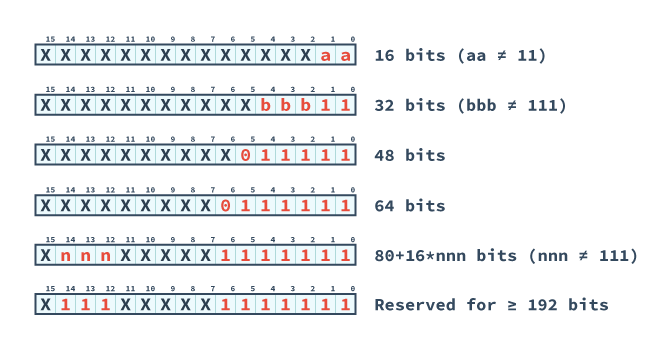
\includegraphics[width=1\linewidth]{images/RV_InstructionLength.png}
    \caption{Codificação de instruções de tamanho variável da arquitetura
                \textit{RISC-V}}\label{fig:riscv_var_length}
\end{figure}

\clearpage

{
    A nomenclatura do conjunto de instruções implementado segue a
    seguinte estrutura:
}

\begin{itemize}[leftmargin=20mm]
    \item {As letras ``RV'';}
    \item {A largura dos registradores do módulo Inteiro;}
    \item {A letra ``I'' representando a base Inteira. Caso o subconjunto
            Embarcado (\textit{Embedded}) seja implementado, substitui-se
            pela letra ``E'';}
    \item {Demais letras identificadoras de módulos opcionais.}
\end{itemize}

{
    Assim, uma implementação com registradores de 64 bits somente com o
    módulo base de Inteiros é denominado ``RV64I''.
}

\section{Módulo Inteiro}
{
    O módulo Inteiro é o módulo base da arquiterura. O \textit{design} de sua
    especificação visa reduzir o \textit{hardware} necesário para uma
    implementação mínima, bem como ser um alvo de compilação satisfatório.
}

{
    Diferente de outras arquiteturas como a \textit{ARM}, as instruções de 
    multiplicação e divisão não fazem parte do conjunto básico uam vez que
    necessitam de circuito especializado e por isso encarecem o desenvolvimento
    e produção dos processadores.
}

{
    Para sistemas embarcados com restrições mais severas de tamanho, custo,
    potência, etc o módulo base I pode ser substituído por um \textit{subset},
    o módulo E. Porém, nenhuma das demais extensões pode ser usada em conjunto
    com o módulo E.
}


\section{Extensões}
    \subsection{Extensão M}
    {
        A extensão M implementa as operações de multiplicação e divisão de
        números inteiros.
    }

    \subsection{Extensão A}
    {
        A extensão A implementa instruções de acesso atômico a memória.
        Instruções atômicas mantém a coerência da memória em sistemas
        preemptivos e paralelos.
    }

    \subsection{Extensão F}
    {
        A extensão F implementa as isntruções de ponto flutuante IEEE 754 de
        precisão simples, bem como o banco de registradores especializado para
        operações com ponto flutuante.
    }

    \subsection{Extensão D}
    {
        A extensão D implementa as instruções de ponto flutuante IEEE 754 de
        precisão dupla. Ela é um incremento à extensão F, sendo esta de
        implementação obrigatória para se poder implementar a extensão D.
    }

    \subsection{Outras Extensões}
    {
        Outras extensões são previstas na especificação da arquitetura, e.g.
        a extensão C para instruções comprimidas (16 bits).
    }

    {
        A arquitetura prevê a expansão de extensões, com alguns
        \textit{opcodes} sendo reservados para essa finalidade. Desse modo,
        instruções proprietárias e/ou customisadas podem ser adicionadas.
    }

\section{Arquitetura Privilegiada}
{
    Para a \textit{ISA RISC-V}, existem quatro níveis de privilégio de acesso,
    sendo eles o de usuário (módulo I e extensões), de máquina 
    (\textit{syscalls}) de supervisor (sistema operacional) e hipervisor
    (virtualização).
}

\section{Formatos de Instruções}
{
    As instruções da arquitetura podem ser separadas em subgrupos de acordo com
    os operadores necessários para o processador interpretá-la. A 
    Figura~\ref{fig:riscv_formats} apresenta os formatos das instruções do
    módulo I da \textit{ISA RISC-V}, e, para efeitos de comparação, a
    Figura~\ref{fig:mips_formats} mostra os formatos de instruções equivalentes
    na arquitetura MIPS32.
}

\begin{figure}[H]
\centering
    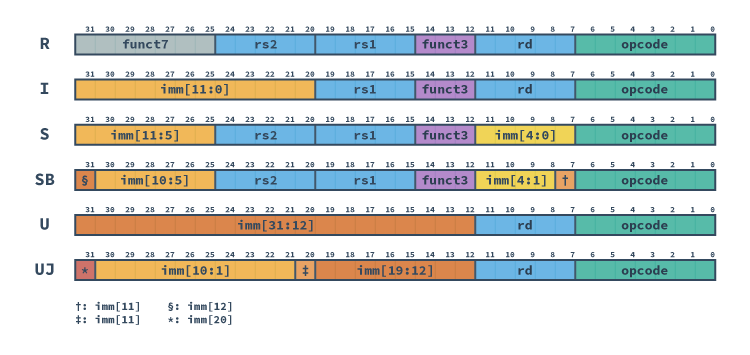
\includegraphics[width=1\linewidth]{images/RV_Formats.png}
    \caption{Formatos de Instruções da\textit{ISA RISC-V}
        }\label{fig:riscv_formats}
\end{figure}

\begin{figure}[H]
\centering
    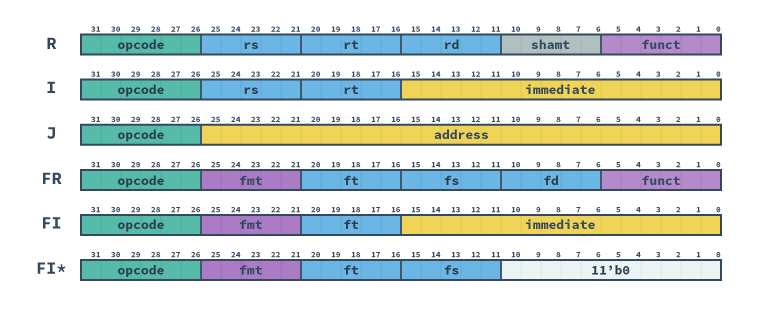
\includegraphics[width=1\linewidth]{images/MIPS_Formats.png}
    \caption{Formatos de Instruções da \textit{ISA MIPS32}
        }\label{fig:mips_formats}
\end{figure}

\section{Formatos de Imediatos}
{
    Os imediatos são operandos descritos na própria instrução em vez de estar
    contido em um registrador. Como os operandos necessitam ter a mesma largura
    que o banco de registradores, algumas regras são utilizadas para gerar os
    operandos imediatos. As figuras a seguir mostram a formação de cada tipo de
    imediato dos formatos da Figura~\ref{fig:riscv_formats}.
}

\begin{figure}[H]
\centering
    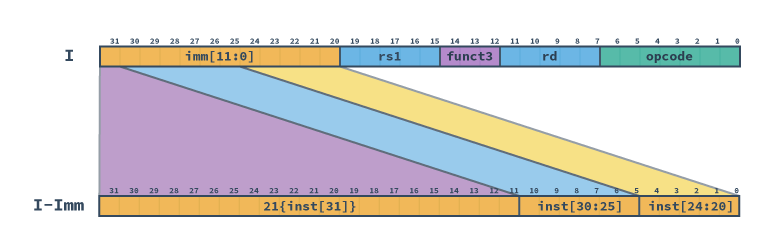
\includegraphics[width=1\linewidth]{images/RV_I_Imm.png}
    \caption{Formação do Imediato de tipo I
        }\label{fig:riscv_i_imm}
\end{figure}

\begin{figure}[H]
\centering
    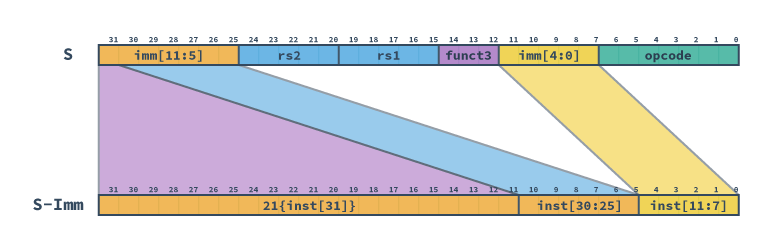
\includegraphics[width=1\linewidth]{images/RV_S_Imm.png}
    \caption{Formação do Imediato de tipo S
        }\label{fig:riscv_s_imm}
\end{figure}

\begin{figure}[H]
\centering
    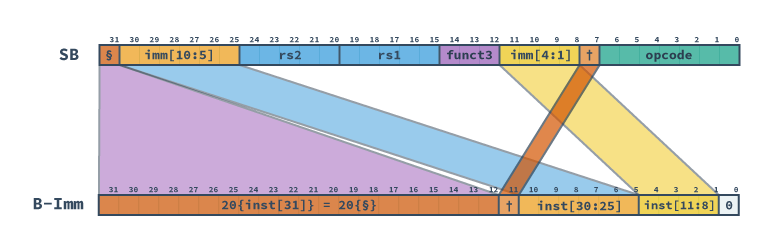
\includegraphics[width=1\linewidth]{images/RV_B_Imm.png}
    \caption{Formação do Imediato de tipo B
        }\label{fig:riscv_b_imm}
\end{figure}

\begin{figure}[H]
\centering
    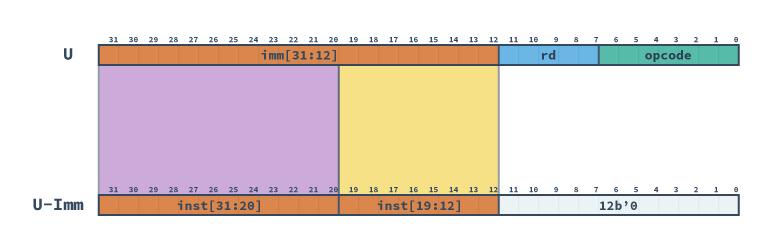
\includegraphics[width=1\linewidth]{images/RV_U_Imm.png}
    \caption{Formação do Imediato de tipo U
        }\label{fig:riscv_u_imm}
\end{figure}

\begin{figure}[H]
\centering
    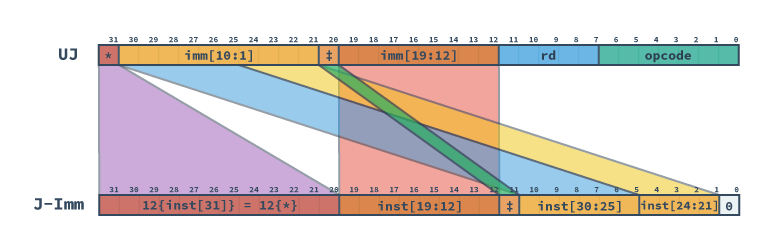
\includegraphics[width=1\linewidth]{images/RV_J_Imm.png}
    \caption{Formação do Imediato de tipo J
        }\label{fig:riscv_j_imm}
\end{figure}

{
    Para efeitos comparativos, a Figura~\ref{fig:mips_immediates} mostra a
    formação de imediatos na arquitetura MIPS32.
}

\begin{figure}[H]
\centering
    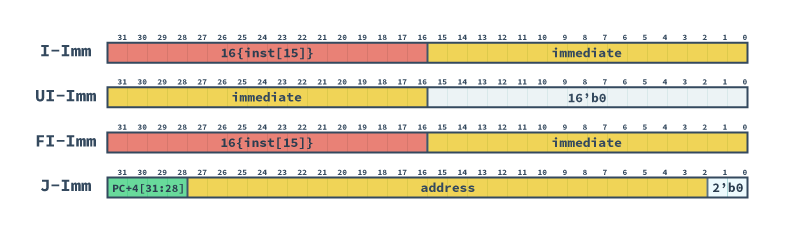
\includegraphics[width=1\linewidth]{images/MIPS_Immediates.png}
    \caption{Formatos de Imediato da \textit{ISA MIPS32}}\label{fig:mips_immediates}
\end{figure}


\chapter{Implementação}\label{CapImpl}

%\resumodocapitulo{Resumo opcional}

\section{Caminho de Dados}
{
    O caminho de dados projetado para a implementação da microarquitetura
    uniciclo é apresentado na Figura~\ref{fig:datapath}.
}

\begin{figure}[H]
\centering
    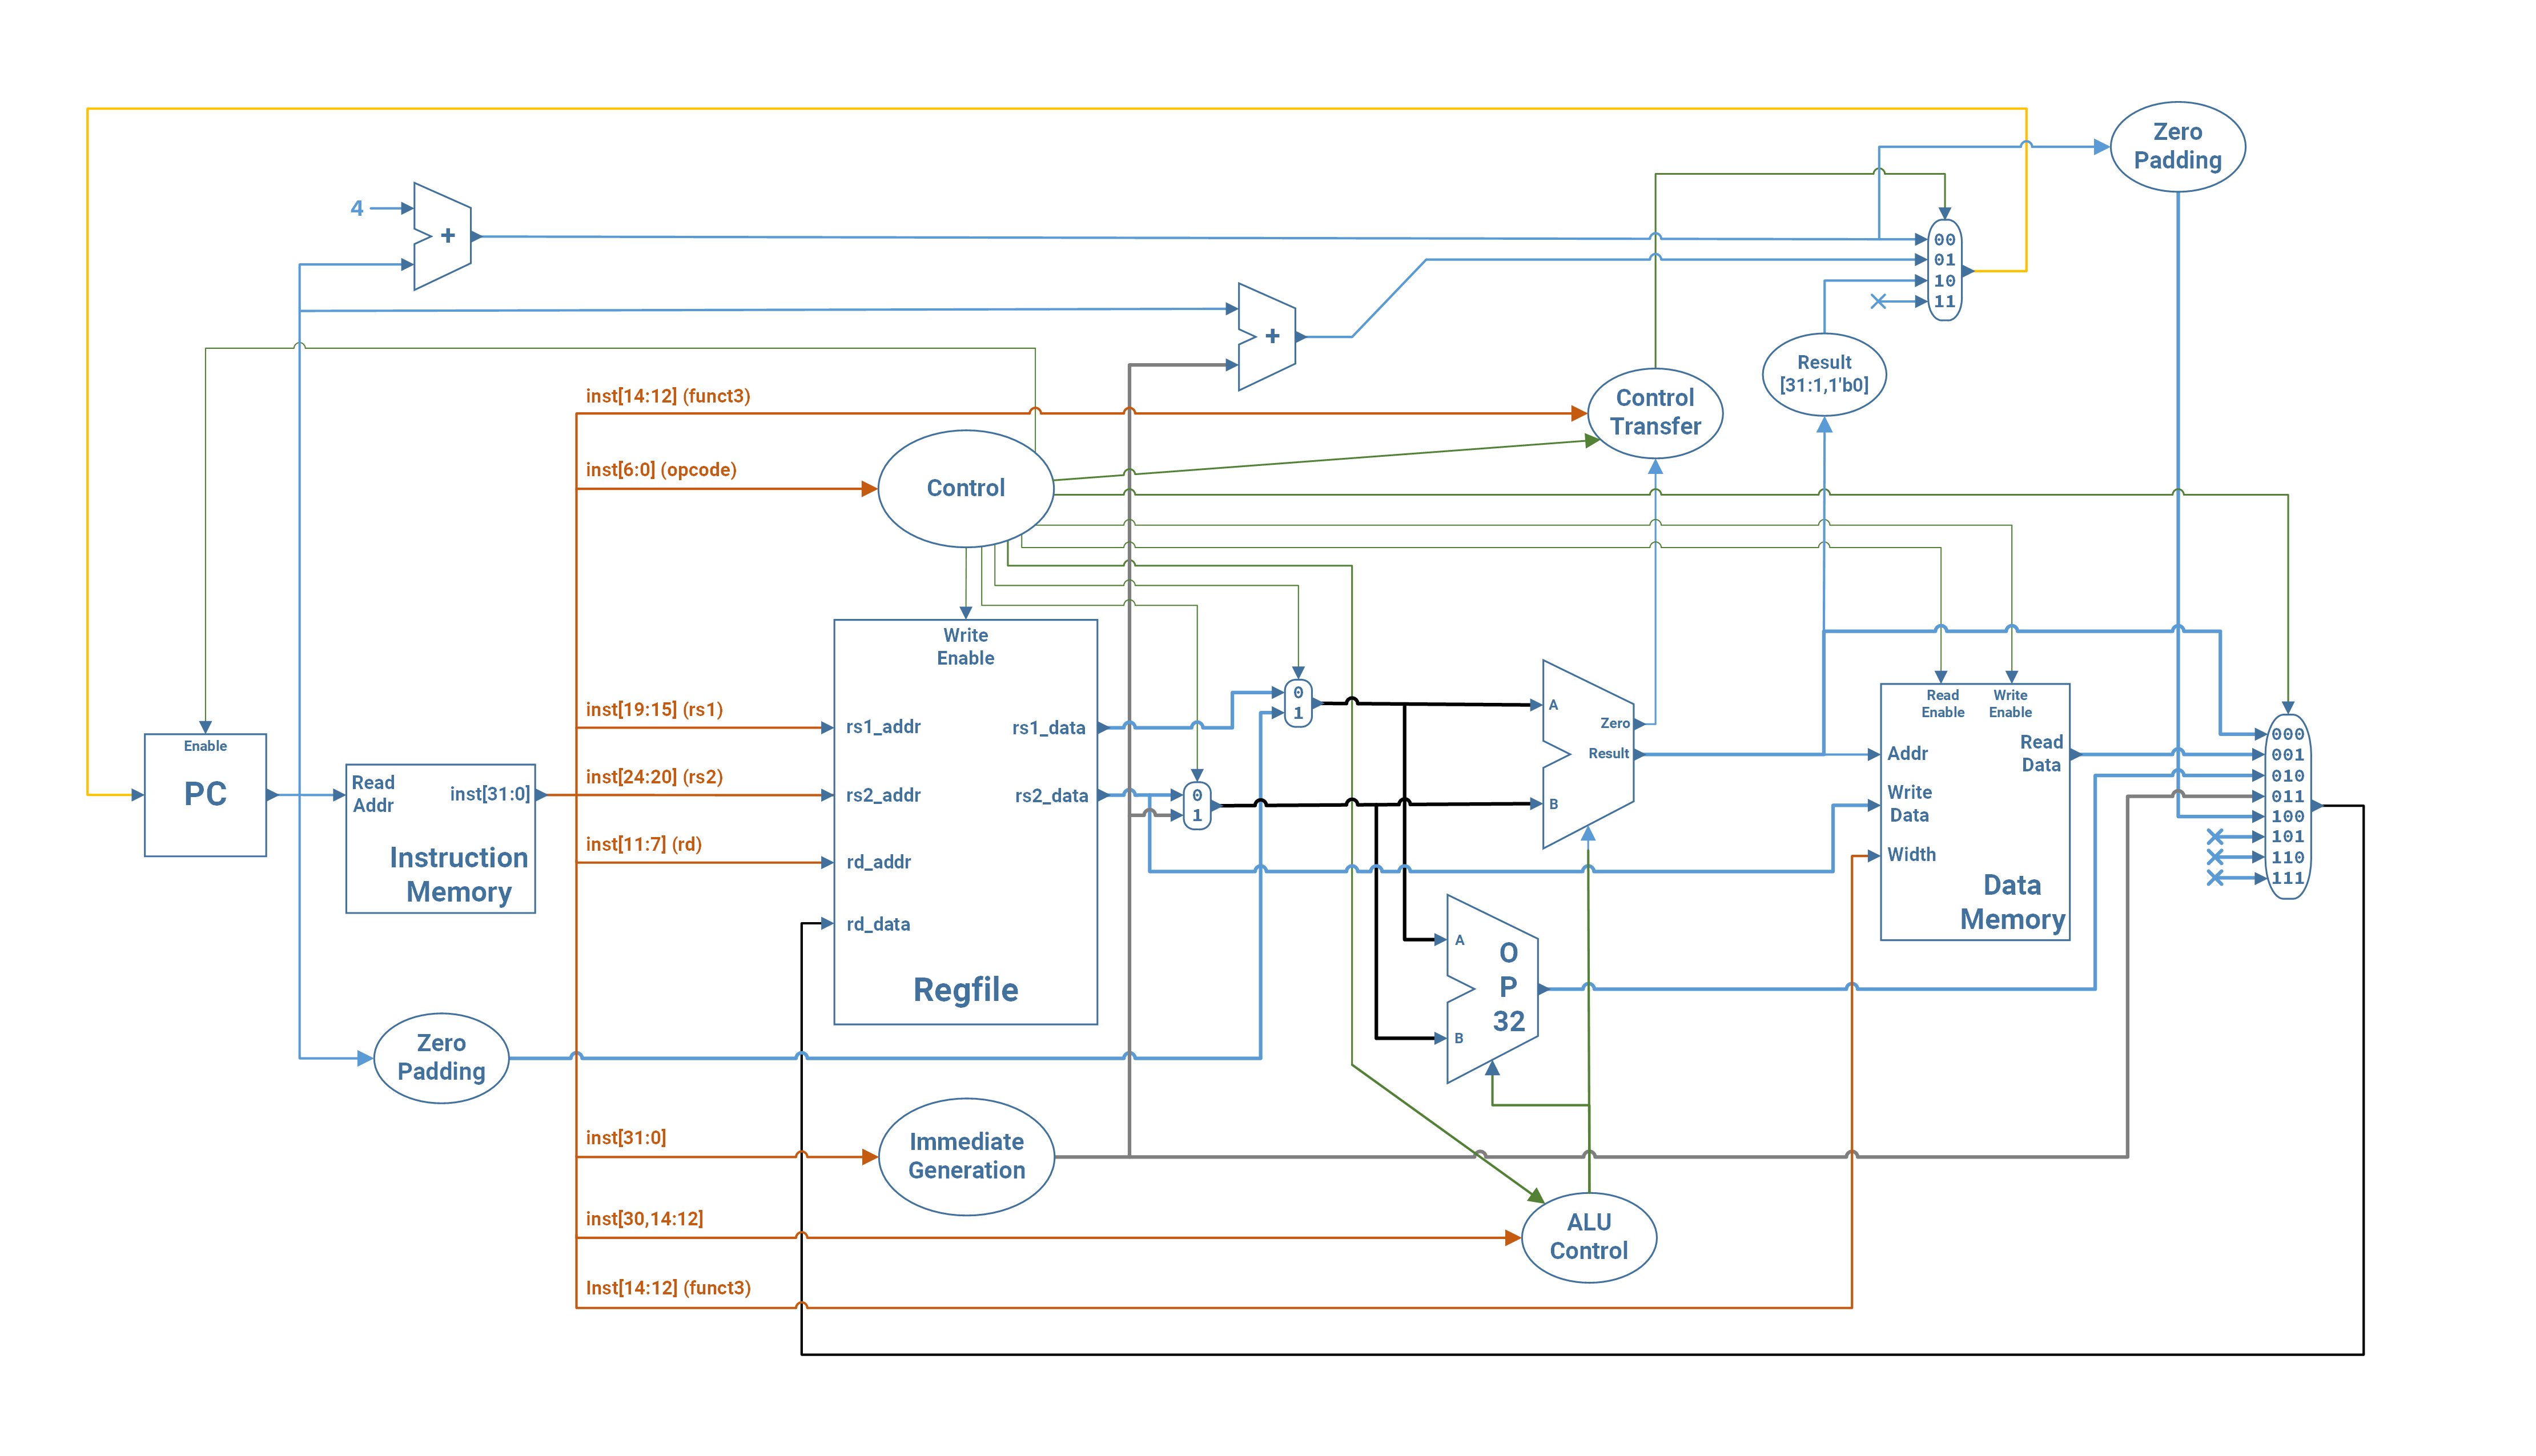
\includegraphics[width=1\linewidth]{images/singlecycle.png}
    \caption{Caminho de Dados implementado para o
                módulo I}\label{fig:datapath}
\end{figure}

{
    O \textit{datapath} possui um banco de 32 registradores de uso geral
    de 64 bits cada. A memória possui arquitetura Harvard, sendo a memória
    de instruções (\textit{text}) \textit{read-only} e a memória de dados
    (\textit{data}) \textit{read-write}.
    São implementadas 49 instruções, sendo elas:
}

\begin{itemize}[leftmargin=20mm]
    \item {LUI:\@ Load Upper Intermediate;}
    \item {AUIPC:\@ Add Upper Intermediate to Program Counter;}
    \item {JAL:\@ Jump And Link;}
    \item {JALR:\@ Jump And Link Register;}
    \item {BEQ:\@ Branch if EQual;}
    \item {BNE:\@ Branch if Not Equal;}
    \item {BLT:\@ Branch if Less Than;}
    \item {BGE:\@ Branch if Greater or Equal;}
    \item {BLTU:\@ Branch if Less Than Unsigned;}
    \item {BGEU:\@ Branch if Greater or Equal Unsigned;}
    \item {LB:\@ Load Byte;}
    \item {LH:\@ Load Halfword;}
    \item {LW:\@ Load Word;}
    \item {LBU:\@ Load Byte Unsigned;}
    \item {LHU:\@ Load Halfword Unsigned;}
    \item {SB:\@ Store Byte;}
    \item {SH:\@ Store Halfword;}
    \item {SW:\@ Store Word;}
    \item {ADDI:\@ ADD Immediate;}
    \item {SLTI:\@ Set on Less Than;}
    \item {SLTIU:\@ Set on Less Than Unsigned;}
    \item {XORI:\@ XOR Immediate;}
    \item {ORI:\@ OR Immediate;}
    \item {ANDI:\@ AND Immediate;}
    \item {SLLI:\@ Shift Left Logical Immedate;}
    \item {SRLI:\@ Shift Right Logical Immediate;}
    \item {SRAI:\@ Shift Right Arithmetic Immediate;}
    \item {ADD:\@ ADD;}
    \item {SUB:\@ SUB;}
    \item {SLL:\@ Shift Left Logical;}
    \item {SLT:\@ Set on Less Than;}
    \item {SLTU:\@ Set on Less Than Unsigned;}
    \item {XOR:\@ XOR;}
    \item {SRL:\@ Shift Right Logical;}
    \item {SRA:\@ Shift Right Arithmetic;}
    \item {OR:\@ OR;}
    \item {AND:\@ AND;}
    \item {LWU:\@ Load Word Unsigned;}
    \item {LD:\@ Load Double;}
    \item {SD:\@ Store Double;}
    \item {ADDIW:\@ ADD Immediate Word-size;}
    \item {SLLIW:\@ Shift Left Logical Immedate Word-size;}
    \item {SRLIW:\@ Shift Right Logical Immediate Word-size;}
    \item {SRAIW:\@ Shift Right Arithmetic Immediate Word-size;}
    \item {ADDW:\@ ADD Word-size;}
    \item {SUBW:\@ SUB Word-size;}
    \item {SLLW:\@ Shift Left Logical Word-size;}
    \item {SRLW:\@ Shift Right Logical Word-size;}
    \item {SRAW:\@ Shift Right Arithmetic Word-size;}
\end{itemize}

{
    Para que o processador seja completamente compatível com a
    especificação da \textit{ISA}, falta implementar tratamentos de
    exceções, interrupções e \textit{traps}, Registradores \textit{CSR},
    instruções de chamada ao ambiente (ECALL/EBREAK), instruções de
    \textit{fencing} de memória, suporte ao acesso desalinhado à memória
    de dados e pilha de endereço de retorno (RAS).
}

\section{\textit{Hardware Description Language}}
{
    Linguagens de Descrição de Hardware, ou \textit{HDL's} são linguagens de
    programação que permitem a descrição em alto nível de um circuito lógico.
}

{
    Diferente de diagramas de blocos onde se descreve o circuito a nível de
    portas lógicas, em uma \textit{HDL} o comportamento do circuito é descrito
    por funções, e um sintetizador de \textit{hardware} (programa similar a um 
    compilador) transforma as funções em circuitos.
}

{
    O uso de \textit{HDL's} possui muitas vantagens em relação aos diagramas de
    blocos. Por se tratar de uma linguagem com maior nível de abstração, o
    entendimento das lógicas de funcionamento se um circuito são mais fáceis de
    se entender, alem de permitir o uso de sistemas de versionamento de código
    e.g.\ git para manter um histórico de todas as alterações feitas.
}

{
    O código a seguir foi retirado do módulo de transferência de controle do 
    processador e exemplifica a estrutura de um programa em Verilog, a 
    linguagem de descrição de \textit{hardware} utilizada no projeto:
}

\begin{lstlisting}[style={verilog-style}]
module control_transfer_singlecycle (
    input  branch_en,
    input  jal_en,
    input  jalr_en,
    input  result_eq_zero,
    input  [2:0] inst_funct3,

    output reg [1:0] pc_sel
);

always @ ( * ) begin
    if (branch_en) begin
        case (inst_funct3)
            `BRANCH_EQ:
                pc_sel = result_eq_zero ? 2'b01 : 2'b00;

            `BRANCH_NE:
                pc_sel = result_eq_zero ? 2'b00 : 2'b01;

            `BRANCH_LT:
                pc_sel = result_eq_zero ? 2'b00 : 2'b01;

            `BRANCH_GE:
                pc_sel = result_eq_zero ? 2'b01 : 2'b00;

            `BRANCH_LTU:
                pc_sel = result_eq_zero ? 2'b00 : 2'b01;

            `BRANCH_GEU:
                pc_sel = result_eq_zero ? 2'b01 : 2'b00;

            default:
                pc_sel = 2'b00;
        endcase
    end

    else if (jal_en) begin
        pc_sel = 2'b01;
    end

    else if (jalr_en) begin
        pc_sel = 2'b10;
    end

    else begin
        pc_sel = 2'b00;
    end
end

endmodule

\end{lstlisting}

\section{\textit{Field Programmable Gate Array}}
{
    As \textit{FPGA's} são circuitos integrados que possuem uma matriz de
    blocos lógicos configuráveis. Um diagrama de blocos ou uma \textit{HDL},
    após passar pelo processo de síntese (transformação em uma linguagem
    intermediária que representa o circuito a nível \textit{TTL}) passa pelos
    processos de mapeamento e alocação (\textit{mapping} e \textit{fitting})
    que conectam os elementos da matriz. Assim, o código ou diagrama são
    ``traduzidos'' em um circuito.
}

\begin{figure}[H]
\centering
    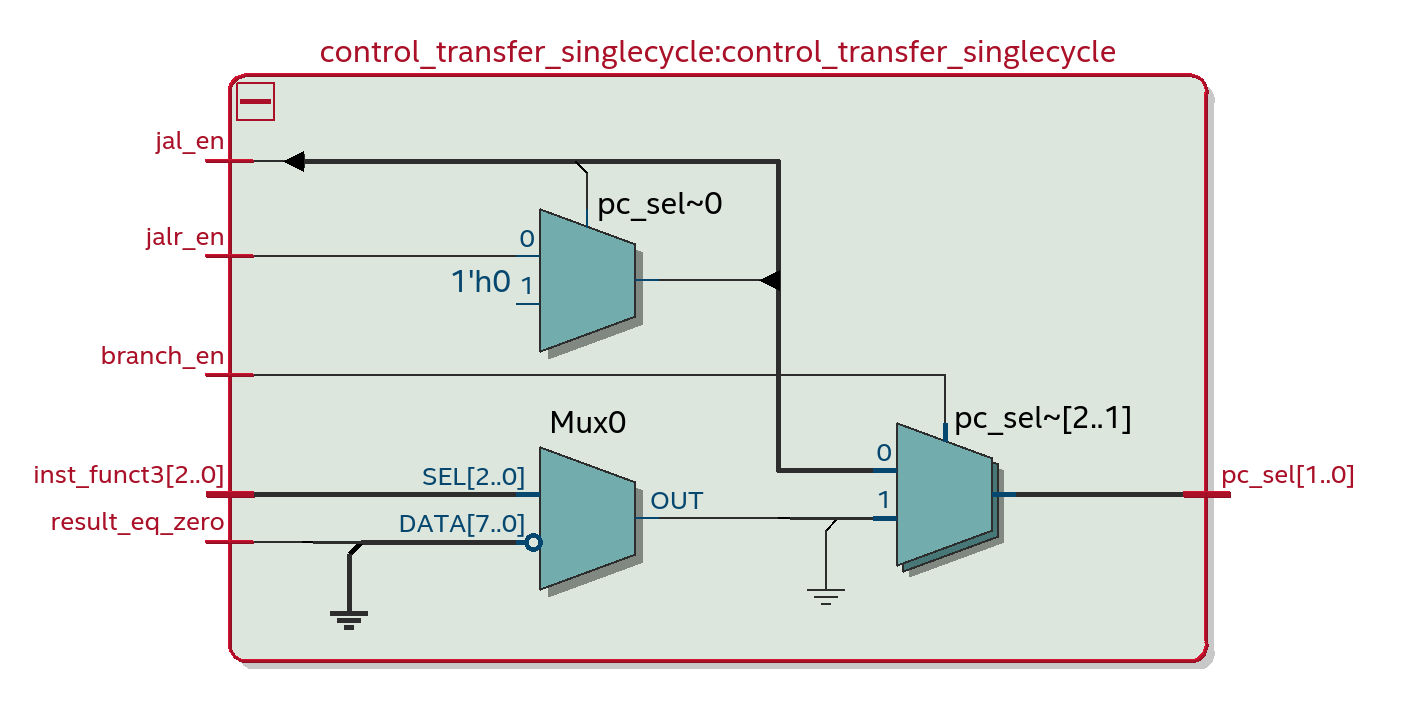
\includegraphics[width=1\linewidth]{images/riscv_sinth.png}
    \caption{Módulo de Transferência de Controle após ser sintetizado
                }\label{fig:riscv_sinth}
\end{figure}

{
    \textit{Kits} de desenvolvimento possuem, além da \textit{FPGA}, diversos
    periféricos conectados a ela, permitindo interfacear o circuito sinteitzado
    com saídas de vídeo, portas USB, memórias FLASH, entre outros componentes.
    A Figura~\ref{fig:DE2_115} apresenta a placa de desenvolvimento DE2-115
    produzida pela empresa \textit{terasIC}.
}

\begin{figure}[H]
\centering
    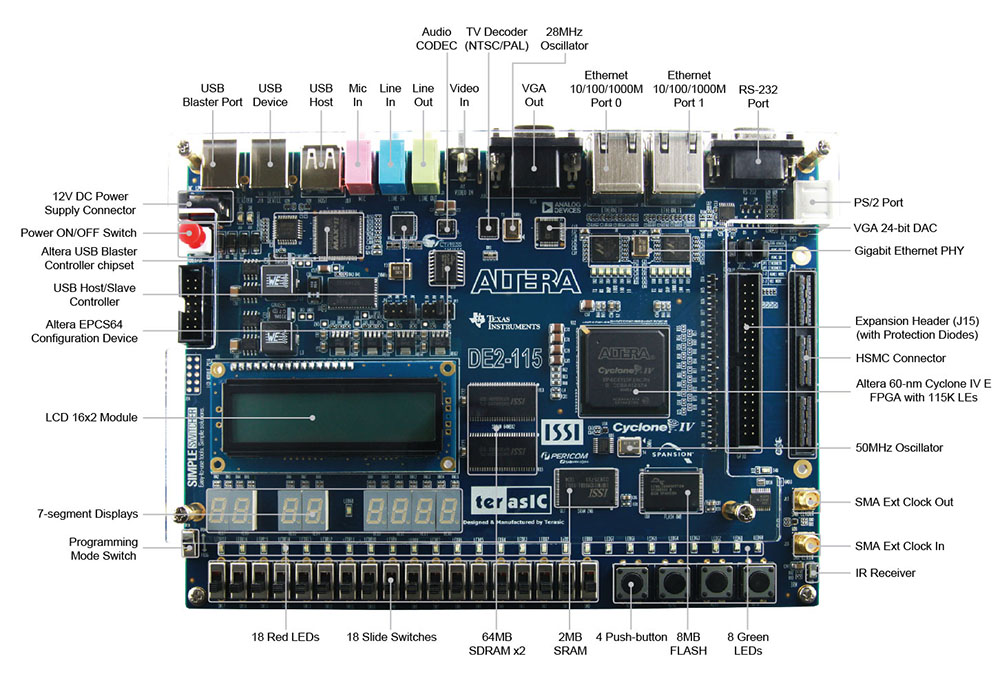
\includegraphics[width=1\linewidth]{images/DE2_115.jpg}
    \caption{Placa de desenvolvimento DE2-115 da terasIC
                }\label{fig:DE2_115}
\end{figure}


\chapter{Resultados}\label{CapResult}

% Resumo opcional. Comentar se não usar.
%\resumodocapitulo{Resumo opcional}


\chapter{Conclusões}

\label{CapConclusoes}

Concluir


\section{Perspectivas Futuras}

Perspectivas futuras



% Bibliografia
\renewcommand{\bibname}{REFERÊNCIAS BIBLIOGRÁFICAS}
\addcontentsline{toc}{chapter}{REFERÊNCIAS BIBLIOGRÁFICAS}


\bibliographystyle{abnt-num}
\bibliography{src/relatorio}


% Anexos
\anexos{}
\makeatletter
\renewcommand{\@makechapterhead}[1]{
  { \parindent\z@ \raggedleft\setfontarial\bfseries
    \LARGE \thechapter. \space\space \uppercase{#1}\par \vskip 40\p@
  }
}
\makeatother


% Anexo I: Descrição do CD

\chapter{Descrição do conteúdo do CD}

\label{AnCD}

Descrever CD.


\refstepcounter{noAnexo}


% Anexo II: Programas Utilizados

\chapter{Programas utilizados}

Quais programas foram utilizados?


\refstepcounter{noAnexo}


% Acrescente mais anexos conforme julgar necessário.

\end{document}
